\documentclass[11pt]{article}

    \usepackage[breakable]{tcolorbox}
    \usepackage{parskip} % Stop auto-indenting (to mimic markdown behaviour)
    
    \usepackage{iftex}
    \ifPDFTeX
    	\usepackage[T1]{fontenc}
    	\usepackage{mathpazo}
    \else
    	\usepackage{fontspec}
    \fi

    % Basic figure setup, for now with no caption control since it's done
    % automatically by Pandoc (which extracts ![](path) syntax from Markdown).
    \usepackage{graphicx}
    % Maintain compatibility with old templates. Remove in nbconvert 6.0
    \let\Oldincludegraphics\includegraphics
    % Ensure that by default, figures have no caption (until we provide a
    % proper Figure object with a Caption API and a way to capture that
    % in the conversion process - todo).
    \usepackage{caption}
    \DeclareCaptionFormat{nocaption}{}
    \captionsetup{format=nocaption,aboveskip=0pt,belowskip=0pt}

    \usepackage[Export]{adjustbox} % Used to constrain images to a maximum size
    \adjustboxset{max size={0.9\linewidth}{0.9\paperheight}}
    \usepackage{float}
    \floatplacement{figure}{H} % forces figures to be placed at the correct location
    \usepackage{xcolor} % Allow colors to be defined
    \usepackage{enumerate} % Needed for markdown enumerations to work
    \usepackage{geometry} % Used to adjust the document margins
    \usepackage{amsmath} % Equations
    \usepackage{amssymb} % Equations
    \usepackage{textcomp} % defines textquotesingle
    % Hack from http://tex.stackexchange.com/a/47451/13684:
    \AtBeginDocument{%
        \def\PYZsq{\textquotesingle}% Upright quotes in Pygmentized code
    }
    \usepackage{upquote} % Upright quotes for verbatim code
    \usepackage{eurosym} % defines \euro
    \usepackage[mathletters]{ucs} % Extended unicode (utf-8) support
    \usepackage{fancyvrb} % verbatim replacement that allows latex
    \usepackage{grffile} % extends the file name processing of package graphics 
                         % to support a larger range
    \makeatletter % fix for grffile with XeLaTeX
    \def\Gread@@xetex#1{%
      \IfFileExists{"\Gin@base".bb}%
      {\Gread@eps{\Gin@base.bb}}%
      {\Gread@@xetex@aux#1}%
    }
    \makeatother

    % The hyperref package gives us a pdf with properly built
    % internal navigation ('pdf bookmarks' for the table of contents,
    % internal cross-reference links, web links for URLs, etc.)
    \usepackage{hyperref}
    % The default LaTeX title has an obnoxious amount of whitespace. By default,
    % titling removes some of it. It also provides customization options.
    \usepackage{titling}
    \usepackage{longtable} % longtable support required by pandoc >1.10
    \usepackage{booktabs}  % table support for pandoc > 1.12.2
    \usepackage[inline]{enumitem} % IRkernel/repr support (it uses the enumerate* environment)
    \usepackage[normalem]{ulem} % ulem is needed to support strikethroughs (\sout)
                                % normalem makes italics be italics, not underlines
    \usepackage{mathrsfs}
    

    
    % Colors for the hyperref package
    \definecolor{urlcolor}{rgb}{0,.145,.698}
    \definecolor{linkcolor}{rgb}{.71,0.21,0.01}
    \definecolor{citecolor}{rgb}{.12,.54,.11}

    % ANSI colors
    \definecolor{ansi-black}{HTML}{3E424D}
    \definecolor{ansi-black-intense}{HTML}{282C36}
    \definecolor{ansi-red}{HTML}{E75C58}
    \definecolor{ansi-red-intense}{HTML}{B22B31}
    \definecolor{ansi-green}{HTML}{00A250}
    \definecolor{ansi-green-intense}{HTML}{007427}
    \definecolor{ansi-yellow}{HTML}{DDB62B}
    \definecolor{ansi-yellow-intense}{HTML}{B27D12}
    \definecolor{ansi-blue}{HTML}{208FFB}
    \definecolor{ansi-blue-intense}{HTML}{0065CA}
    \definecolor{ansi-magenta}{HTML}{D160C4}
    \definecolor{ansi-magenta-intense}{HTML}{A03196}
    \definecolor{ansi-cyan}{HTML}{60C6C8}
    \definecolor{ansi-cyan-intense}{HTML}{258F8F}
    \definecolor{ansi-white}{HTML}{C5C1B4}
    \definecolor{ansi-white-intense}{HTML}{A1A6B2}
    \definecolor{ansi-default-inverse-fg}{HTML}{FFFFFF}
    \definecolor{ansi-default-inverse-bg}{HTML}{000000}

    % commands and environments needed by pandoc snippets
    % extracted from the output of `pandoc -s`
    \providecommand{\tightlist}{%
      \setlength{\itemsep}{0pt}\setlength{\parskip}{0pt}}
    \DefineVerbatimEnvironment{Highlighting}{Verbatim}{commandchars=\\\{\}}
    % Add ',fontsize=\small' for more characters per line
    \newenvironment{Shaded}{}{}
    \newcommand{\KeywordTok}[1]{\textcolor[rgb]{0.00,0.44,0.13}{\textbf{{#1}}}}
    \newcommand{\DataTypeTok}[1]{\textcolor[rgb]{0.56,0.13,0.00}{{#1}}}
    \newcommand{\DecValTok}[1]{\textcolor[rgb]{0.25,0.63,0.44}{{#1}}}
    \newcommand{\BaseNTok}[1]{\textcolor[rgb]{0.25,0.63,0.44}{{#1}}}
    \newcommand{\FloatTok}[1]{\textcolor[rgb]{0.25,0.63,0.44}{{#1}}}
    \newcommand{\CharTok}[1]{\textcolor[rgb]{0.25,0.44,0.63}{{#1}}}
    \newcommand{\StringTok}[1]{\textcolor[rgb]{0.25,0.44,0.63}{{#1}}}
    \newcommand{\CommentTok}[1]{\textcolor[rgb]{0.38,0.63,0.69}{\textit{{#1}}}}
    \newcommand{\OtherTok}[1]{\textcolor[rgb]{0.00,0.44,0.13}{{#1}}}
    \newcommand{\AlertTok}[1]{\textcolor[rgb]{1.00,0.00,0.00}{\textbf{{#1}}}}
    \newcommand{\FunctionTok}[1]{\textcolor[rgb]{0.02,0.16,0.49}{{#1}}}
    \newcommand{\RegionMarkerTok}[1]{{#1}}
    \newcommand{\ErrorTok}[1]{\textcolor[rgb]{1.00,0.00,0.00}{\textbf{{#1}}}}
    \newcommand{\NormalTok}[1]{{#1}}
    
    % Additional commands for more recent versions of Pandoc
    \newcommand{\ConstantTok}[1]{\textcolor[rgb]{0.53,0.00,0.00}{{#1}}}
    \newcommand{\SpecialCharTok}[1]{\textcolor[rgb]{0.25,0.44,0.63}{{#1}}}
    \newcommand{\VerbatimStringTok}[1]{\textcolor[rgb]{0.25,0.44,0.63}{{#1}}}
    \newcommand{\SpecialStringTok}[1]{\textcolor[rgb]{0.73,0.40,0.53}{{#1}}}
    \newcommand{\ImportTok}[1]{{#1}}
    \newcommand{\DocumentationTok}[1]{\textcolor[rgb]{0.73,0.13,0.13}{\textit{{#1}}}}
    \newcommand{\AnnotationTok}[1]{\textcolor[rgb]{0.38,0.63,0.69}{\textbf{\textit{{#1}}}}}
    \newcommand{\CommentVarTok}[1]{\textcolor[rgb]{0.38,0.63,0.69}{\textbf{\textit{{#1}}}}}
    \newcommand{\VariableTok}[1]{\textcolor[rgb]{0.10,0.09,0.49}{{#1}}}
    \newcommand{\ControlFlowTok}[1]{\textcolor[rgb]{0.00,0.44,0.13}{\textbf{{#1}}}}
    \newcommand{\OperatorTok}[1]{\textcolor[rgb]{0.40,0.40,0.40}{{#1}}}
    \newcommand{\BuiltInTok}[1]{{#1}}
    \newcommand{\ExtensionTok}[1]{{#1}}
    \newcommand{\PreprocessorTok}[1]{\textcolor[rgb]{0.74,0.48,0.00}{{#1}}}
    \newcommand{\AttributeTok}[1]{\textcolor[rgb]{0.49,0.56,0.16}{{#1}}}
    \newcommand{\InformationTok}[1]{\textcolor[rgb]{0.38,0.63,0.69}{\textbf{\textit{{#1}}}}}
    \newcommand{\WarningTok}[1]{\textcolor[rgb]{0.38,0.63,0.69}{\textbf{\textit{{#1}}}}}
    
    
    % Define a nice break command that doesn't care if a line doesn't already
    % exist.
    \def\br{\hspace*{\fill} \\* }
    % Math Jax compatibility definitions
    \def\gt{>}
    \def\lt{<}
    \let\Oldtex\TeX
    \let\Oldlatex\LaTeX
    \renewcommand{\TeX}{\textrm{\Oldtex}}
    \renewcommand{\LaTeX}{\textrm{\Oldlatex}}
    % Document parameters
    % Document title
    \title{Dimensionality Reduction}
    
    
    
    
    
% Pygments definitions
\makeatletter
\def\PY@reset{\let\PY@it=\relax \let\PY@bf=\relax%
    \let\PY@ul=\relax \let\PY@tc=\relax%
    \let\PY@bc=\relax \let\PY@ff=\relax}
\def\PY@tok#1{\csname PY@tok@#1\endcsname}
\def\PY@toks#1+{\ifx\relax#1\empty\else%
    \PY@tok{#1}\expandafter\PY@toks\fi}
\def\PY@do#1{\PY@bc{\PY@tc{\PY@ul{%
    \PY@it{\PY@bf{\PY@ff{#1}}}}}}}
\def\PY#1#2{\PY@reset\PY@toks#1+\relax+\PY@do{#2}}

\expandafter\def\csname PY@tok@w\endcsname{\def\PY@tc##1{\textcolor[rgb]{0.73,0.73,0.73}{##1}}}
\expandafter\def\csname PY@tok@c\endcsname{\let\PY@it=\textit\def\PY@tc##1{\textcolor[rgb]{0.25,0.50,0.50}{##1}}}
\expandafter\def\csname PY@tok@cp\endcsname{\def\PY@tc##1{\textcolor[rgb]{0.74,0.48,0.00}{##1}}}
\expandafter\def\csname PY@tok@k\endcsname{\let\PY@bf=\textbf\def\PY@tc##1{\textcolor[rgb]{0.00,0.50,0.00}{##1}}}
\expandafter\def\csname PY@tok@kp\endcsname{\def\PY@tc##1{\textcolor[rgb]{0.00,0.50,0.00}{##1}}}
\expandafter\def\csname PY@tok@kt\endcsname{\def\PY@tc##1{\textcolor[rgb]{0.69,0.00,0.25}{##1}}}
\expandafter\def\csname PY@tok@o\endcsname{\def\PY@tc##1{\textcolor[rgb]{0.40,0.40,0.40}{##1}}}
\expandafter\def\csname PY@tok@ow\endcsname{\let\PY@bf=\textbf\def\PY@tc##1{\textcolor[rgb]{0.67,0.13,1.00}{##1}}}
\expandafter\def\csname PY@tok@nb\endcsname{\def\PY@tc##1{\textcolor[rgb]{0.00,0.50,0.00}{##1}}}
\expandafter\def\csname PY@tok@nf\endcsname{\def\PY@tc##1{\textcolor[rgb]{0.00,0.00,1.00}{##1}}}
\expandafter\def\csname PY@tok@nc\endcsname{\let\PY@bf=\textbf\def\PY@tc##1{\textcolor[rgb]{0.00,0.00,1.00}{##1}}}
\expandafter\def\csname PY@tok@nn\endcsname{\let\PY@bf=\textbf\def\PY@tc##1{\textcolor[rgb]{0.00,0.00,1.00}{##1}}}
\expandafter\def\csname PY@tok@ne\endcsname{\let\PY@bf=\textbf\def\PY@tc##1{\textcolor[rgb]{0.82,0.25,0.23}{##1}}}
\expandafter\def\csname PY@tok@nv\endcsname{\def\PY@tc##1{\textcolor[rgb]{0.10,0.09,0.49}{##1}}}
\expandafter\def\csname PY@tok@no\endcsname{\def\PY@tc##1{\textcolor[rgb]{0.53,0.00,0.00}{##1}}}
\expandafter\def\csname PY@tok@nl\endcsname{\def\PY@tc##1{\textcolor[rgb]{0.63,0.63,0.00}{##1}}}
\expandafter\def\csname PY@tok@ni\endcsname{\let\PY@bf=\textbf\def\PY@tc##1{\textcolor[rgb]{0.60,0.60,0.60}{##1}}}
\expandafter\def\csname PY@tok@na\endcsname{\def\PY@tc##1{\textcolor[rgb]{0.49,0.56,0.16}{##1}}}
\expandafter\def\csname PY@tok@nt\endcsname{\let\PY@bf=\textbf\def\PY@tc##1{\textcolor[rgb]{0.00,0.50,0.00}{##1}}}
\expandafter\def\csname PY@tok@nd\endcsname{\def\PY@tc##1{\textcolor[rgb]{0.67,0.13,1.00}{##1}}}
\expandafter\def\csname PY@tok@s\endcsname{\def\PY@tc##1{\textcolor[rgb]{0.73,0.13,0.13}{##1}}}
\expandafter\def\csname PY@tok@sd\endcsname{\let\PY@it=\textit\def\PY@tc##1{\textcolor[rgb]{0.73,0.13,0.13}{##1}}}
\expandafter\def\csname PY@tok@si\endcsname{\let\PY@bf=\textbf\def\PY@tc##1{\textcolor[rgb]{0.73,0.40,0.53}{##1}}}
\expandafter\def\csname PY@tok@se\endcsname{\let\PY@bf=\textbf\def\PY@tc##1{\textcolor[rgb]{0.73,0.40,0.13}{##1}}}
\expandafter\def\csname PY@tok@sr\endcsname{\def\PY@tc##1{\textcolor[rgb]{0.73,0.40,0.53}{##1}}}
\expandafter\def\csname PY@tok@ss\endcsname{\def\PY@tc##1{\textcolor[rgb]{0.10,0.09,0.49}{##1}}}
\expandafter\def\csname PY@tok@sx\endcsname{\def\PY@tc##1{\textcolor[rgb]{0.00,0.50,0.00}{##1}}}
\expandafter\def\csname PY@tok@m\endcsname{\def\PY@tc##1{\textcolor[rgb]{0.40,0.40,0.40}{##1}}}
\expandafter\def\csname PY@tok@gh\endcsname{\let\PY@bf=\textbf\def\PY@tc##1{\textcolor[rgb]{0.00,0.00,0.50}{##1}}}
\expandafter\def\csname PY@tok@gu\endcsname{\let\PY@bf=\textbf\def\PY@tc##1{\textcolor[rgb]{0.50,0.00,0.50}{##1}}}
\expandafter\def\csname PY@tok@gd\endcsname{\def\PY@tc##1{\textcolor[rgb]{0.63,0.00,0.00}{##1}}}
\expandafter\def\csname PY@tok@gi\endcsname{\def\PY@tc##1{\textcolor[rgb]{0.00,0.63,0.00}{##1}}}
\expandafter\def\csname PY@tok@gr\endcsname{\def\PY@tc##1{\textcolor[rgb]{1.00,0.00,0.00}{##1}}}
\expandafter\def\csname PY@tok@ge\endcsname{\let\PY@it=\textit}
\expandafter\def\csname PY@tok@gs\endcsname{\let\PY@bf=\textbf}
\expandafter\def\csname PY@tok@gp\endcsname{\let\PY@bf=\textbf\def\PY@tc##1{\textcolor[rgb]{0.00,0.00,0.50}{##1}}}
\expandafter\def\csname PY@tok@go\endcsname{\def\PY@tc##1{\textcolor[rgb]{0.53,0.53,0.53}{##1}}}
\expandafter\def\csname PY@tok@gt\endcsname{\def\PY@tc##1{\textcolor[rgb]{0.00,0.27,0.87}{##1}}}
\expandafter\def\csname PY@tok@err\endcsname{\def\PY@bc##1{\setlength{\fboxsep}{0pt}\fcolorbox[rgb]{1.00,0.00,0.00}{1,1,1}{\strut ##1}}}
\expandafter\def\csname PY@tok@kc\endcsname{\let\PY@bf=\textbf\def\PY@tc##1{\textcolor[rgb]{0.00,0.50,0.00}{##1}}}
\expandafter\def\csname PY@tok@kd\endcsname{\let\PY@bf=\textbf\def\PY@tc##1{\textcolor[rgb]{0.00,0.50,0.00}{##1}}}
\expandafter\def\csname PY@tok@kn\endcsname{\let\PY@bf=\textbf\def\PY@tc##1{\textcolor[rgb]{0.00,0.50,0.00}{##1}}}
\expandafter\def\csname PY@tok@kr\endcsname{\let\PY@bf=\textbf\def\PY@tc##1{\textcolor[rgb]{0.00,0.50,0.00}{##1}}}
\expandafter\def\csname PY@tok@bp\endcsname{\def\PY@tc##1{\textcolor[rgb]{0.00,0.50,0.00}{##1}}}
\expandafter\def\csname PY@tok@fm\endcsname{\def\PY@tc##1{\textcolor[rgb]{0.00,0.00,1.00}{##1}}}
\expandafter\def\csname PY@tok@vc\endcsname{\def\PY@tc##1{\textcolor[rgb]{0.10,0.09,0.49}{##1}}}
\expandafter\def\csname PY@tok@vg\endcsname{\def\PY@tc##1{\textcolor[rgb]{0.10,0.09,0.49}{##1}}}
\expandafter\def\csname PY@tok@vi\endcsname{\def\PY@tc##1{\textcolor[rgb]{0.10,0.09,0.49}{##1}}}
\expandafter\def\csname PY@tok@vm\endcsname{\def\PY@tc##1{\textcolor[rgb]{0.10,0.09,0.49}{##1}}}
\expandafter\def\csname PY@tok@sa\endcsname{\def\PY@tc##1{\textcolor[rgb]{0.73,0.13,0.13}{##1}}}
\expandafter\def\csname PY@tok@sb\endcsname{\def\PY@tc##1{\textcolor[rgb]{0.73,0.13,0.13}{##1}}}
\expandafter\def\csname PY@tok@sc\endcsname{\def\PY@tc##1{\textcolor[rgb]{0.73,0.13,0.13}{##1}}}
\expandafter\def\csname PY@tok@dl\endcsname{\def\PY@tc##1{\textcolor[rgb]{0.73,0.13,0.13}{##1}}}
\expandafter\def\csname PY@tok@s2\endcsname{\def\PY@tc##1{\textcolor[rgb]{0.73,0.13,0.13}{##1}}}
\expandafter\def\csname PY@tok@sh\endcsname{\def\PY@tc##1{\textcolor[rgb]{0.73,0.13,0.13}{##1}}}
\expandafter\def\csname PY@tok@s1\endcsname{\def\PY@tc##1{\textcolor[rgb]{0.73,0.13,0.13}{##1}}}
\expandafter\def\csname PY@tok@mb\endcsname{\def\PY@tc##1{\textcolor[rgb]{0.40,0.40,0.40}{##1}}}
\expandafter\def\csname PY@tok@mf\endcsname{\def\PY@tc##1{\textcolor[rgb]{0.40,0.40,0.40}{##1}}}
\expandafter\def\csname PY@tok@mh\endcsname{\def\PY@tc##1{\textcolor[rgb]{0.40,0.40,0.40}{##1}}}
\expandafter\def\csname PY@tok@mi\endcsname{\def\PY@tc##1{\textcolor[rgb]{0.40,0.40,0.40}{##1}}}
\expandafter\def\csname PY@tok@il\endcsname{\def\PY@tc##1{\textcolor[rgb]{0.40,0.40,0.40}{##1}}}
\expandafter\def\csname PY@tok@mo\endcsname{\def\PY@tc##1{\textcolor[rgb]{0.40,0.40,0.40}{##1}}}
\expandafter\def\csname PY@tok@ch\endcsname{\let\PY@it=\textit\def\PY@tc##1{\textcolor[rgb]{0.25,0.50,0.50}{##1}}}
\expandafter\def\csname PY@tok@cm\endcsname{\let\PY@it=\textit\def\PY@tc##1{\textcolor[rgb]{0.25,0.50,0.50}{##1}}}
\expandafter\def\csname PY@tok@cpf\endcsname{\let\PY@it=\textit\def\PY@tc##1{\textcolor[rgb]{0.25,0.50,0.50}{##1}}}
\expandafter\def\csname PY@tok@c1\endcsname{\let\PY@it=\textit\def\PY@tc##1{\textcolor[rgb]{0.25,0.50,0.50}{##1}}}
\expandafter\def\csname PY@tok@cs\endcsname{\let\PY@it=\textit\def\PY@tc##1{\textcolor[rgb]{0.25,0.50,0.50}{##1}}}

\def\PYZbs{\char`\\}
\def\PYZus{\char`\_}
\def\PYZob{\char`\{}
\def\PYZcb{\char`\}}
\def\PYZca{\char`\^}
\def\PYZam{\char`\&}
\def\PYZlt{\char`\<}
\def\PYZgt{\char`\>}
\def\PYZsh{\char`\#}
\def\PYZpc{\char`\%}
\def\PYZdl{\char`\$}
\def\PYZhy{\char`\-}
\def\PYZsq{\char`\'}
\def\PYZdq{\char`\"}
\def\PYZti{\char`\~}
% for compatibility with earlier versions
\def\PYZat{@}
\def\PYZlb{[}
\def\PYZrb{]}
\makeatother


    % For linebreaks inside Verbatim environment from package fancyvrb. 
    \makeatletter
        \newbox\Wrappedcontinuationbox 
        \newbox\Wrappedvisiblespacebox 
        \newcommand*\Wrappedvisiblespace {\textcolor{red}{\textvisiblespace}} 
        \newcommand*\Wrappedcontinuationsymbol {\textcolor{red}{\llap{\tiny$\m@th\hookrightarrow$}}} 
        \newcommand*\Wrappedcontinuationindent {3ex } 
        \newcommand*\Wrappedafterbreak {\kern\Wrappedcontinuationindent\copy\Wrappedcontinuationbox} 
        % Take advantage of the already applied Pygments mark-up to insert 
        % potential linebreaks for TeX processing. 
        %        {, <, #, %, $, ' and ": go to next line. 
        %        _, }, ^, &, >, - and ~: stay at end of broken line. 
        % Use of \textquotesingle for straight quote. 
        \newcommand*\Wrappedbreaksatspecials {% 
            \def\PYGZus{\discretionary{\char`\_}{\Wrappedafterbreak}{\char`\_}}% 
            \def\PYGZob{\discretionary{}{\Wrappedafterbreak\char`\{}{\char`\{}}% 
            \def\PYGZcb{\discretionary{\char`\}}{\Wrappedafterbreak}{\char`\}}}% 
            \def\PYGZca{\discretionary{\char`\^}{\Wrappedafterbreak}{\char`\^}}% 
            \def\PYGZam{\discretionary{\char`\&}{\Wrappedafterbreak}{\char`\&}}% 
            \def\PYGZlt{\discretionary{}{\Wrappedafterbreak\char`\<}{\char`\<}}% 
            \def\PYGZgt{\discretionary{\char`\>}{\Wrappedafterbreak}{\char`\>}}% 
            \def\PYGZsh{\discretionary{}{\Wrappedafterbreak\char`\#}{\char`\#}}% 
            \def\PYGZpc{\discretionary{}{\Wrappedafterbreak\char`\%}{\char`\%}}% 
            \def\PYGZdl{\discretionary{}{\Wrappedafterbreak\char`\$}{\char`\$}}% 
            \def\PYGZhy{\discretionary{\char`\-}{\Wrappedafterbreak}{\char`\-}}% 
            \def\PYGZsq{\discretionary{}{\Wrappedafterbreak\textquotesingle}{\textquotesingle}}% 
            \def\PYGZdq{\discretionary{}{\Wrappedafterbreak\char`\"}{\char`\"}}% 
            \def\PYGZti{\discretionary{\char`\~}{\Wrappedafterbreak}{\char`\~}}% 
        } 
        % Some characters . , ; ? ! / are not pygmentized. 
        % This macro makes them "active" and they will insert potential linebreaks 
        \newcommand*\Wrappedbreaksatpunct {% 
            \lccode`\~`\.\lowercase{\def~}{\discretionary{\hbox{\char`\.}}{\Wrappedafterbreak}{\hbox{\char`\.}}}% 
            \lccode`\~`\,\lowercase{\def~}{\discretionary{\hbox{\char`\,}}{\Wrappedafterbreak}{\hbox{\char`\,}}}% 
            \lccode`\~`\;\lowercase{\def~}{\discretionary{\hbox{\char`\;}}{\Wrappedafterbreak}{\hbox{\char`\;}}}% 
            \lccode`\~`\:\lowercase{\def~}{\discretionary{\hbox{\char`\:}}{\Wrappedafterbreak}{\hbox{\char`\:}}}% 
            \lccode`\~`\?\lowercase{\def~}{\discretionary{\hbox{\char`\?}}{\Wrappedafterbreak}{\hbox{\char`\?}}}% 
            \lccode`\~`\!\lowercase{\def~}{\discretionary{\hbox{\char`\!}}{\Wrappedafterbreak}{\hbox{\char`\!}}}% 
            \lccode`\~`\/\lowercase{\def~}{\discretionary{\hbox{\char`\/}}{\Wrappedafterbreak}{\hbox{\char`\/}}}% 
            \catcode`\.\active
            \catcode`\,\active 
            \catcode`\;\active
            \catcode`\:\active
            \catcode`\?\active
            \catcode`\!\active
            \catcode`\/\active 
            \lccode`\~`\~ 	
        }
    \makeatother

    \let\OriginalVerbatim=\Verbatim
    \makeatletter
    \renewcommand{\Verbatim}[1][1]{%
        %\parskip\z@skip
        \sbox\Wrappedcontinuationbox {\Wrappedcontinuationsymbol}%
        \sbox\Wrappedvisiblespacebox {\FV@SetupFont\Wrappedvisiblespace}%
        \def\FancyVerbFormatLine ##1{\hsize\linewidth
            \vtop{\raggedright\hyphenpenalty\z@\exhyphenpenalty\z@
                \doublehyphendemerits\z@\finalhyphendemerits\z@
                \strut ##1\strut}%
        }%
        % If the linebreak is at a space, the latter will be displayed as visible
        % space at end of first line, and a continuation symbol starts next line.
        % Stretch/shrink are however usually zero for typewriter font.
        \def\FV@Space {%
            \nobreak\hskip\z@ plus\fontdimen3\font minus\fontdimen4\font
            \discretionary{\copy\Wrappedvisiblespacebox}{\Wrappedafterbreak}
            {\kern\fontdimen2\font}%
        }%
        
        % Allow breaks at special characters using \PYG... macros.
        \Wrappedbreaksatspecials
        % Breaks at punctuation characters . , ; ? ! and / need catcode=\active 	
        \OriginalVerbatim[#1,codes*=\Wrappedbreaksatpunct]%
    }
    \makeatother

    % Exact colors from NB
    \definecolor{incolor}{HTML}{303F9F}
    \definecolor{outcolor}{HTML}{D84315}
    \definecolor{cellborder}{HTML}{CFCFCF}
    \definecolor{cellbackground}{HTML}{F7F7F7}
    
    % prompt
    \makeatletter
    \newcommand{\boxspacing}{\kern\kvtcb@left@rule\kern\kvtcb@boxsep}
    \makeatother
    \newcommand{\prompt}[4]{
        \ttfamily\llap{{\color{#2}[#3]:\hspace{3pt}#4}}\vspace{-\baselineskip}
    }
    

    
    % Prevent overflowing lines due to hard-to-break entities
    \sloppy 
    % Setup hyperref package
    \hypersetup{
      breaklinks=true,  % so long urls are correctly broken across lines
      colorlinks=true,
      urlcolor=urlcolor,
      linkcolor=linkcolor,
      citecolor=citecolor,
      }
    % Slightly bigger margins than the latex defaults
    
    \geometry{verbose,tmargin=1in,bmargin=1in,lmargin=1in,rmargin=1in}
    
    

\begin{document}
    
    \maketitle
    
    

    
    \hypertarget{dimensionality-reduction}{%
\section{Dimensionality Reduction}\label{dimensionality-reduction}}

    The complexity of any classifier or regressor depends on the number of
inputs (Both number of samples and features), this determines the time
and space complexity of the classifier or regressor. So feature
selection (Of which dimensionality reduction is a subset) becomes an
important part of the decision making process.

    Feature selection, ideally, should not be a seperate process and should
infact be a part of the decision making algorithm. 1. The complexity of
most learning algorithms depend on the number of input samples N, and
the dimensions of these samples D.So reducing these implies a direct
reduction in time and space complexity of the algorithm. Reducing the
dimensions D, also reduces the inference complexity during test times.
This also, to a certain extent, helps explain the process of decision
making better (Not always). 2. In case of feature extraction. If, for
some reason, we decide to exclude feature, we then save the cost of
extracting said feature making the pipeline (Of decision making) more
efficient. 3. Lower dimensions ensures less chances of overfitting
(Usually) and hence a decision maing process that is explainable by only
a few features is more robust (For smaller datasets) 4. Having lower
dimensions help visualization and detecting structure of the data which
could prove useful for outlier detection.

    \hypertarget{multi-dimensional-scaling}{%
\section{Multi-Dimensional Scaling}\label{multi-dimensional-scaling}}

    Multi domensional scaling aims to map the features from an unknown
dimensional space to a N dimensional space. Consider N points in the
data. The dimesnionality of these data points are unknown. Distance
\(d_{ij}\), for all points i , j where i , j = 1 , 2 , .. N , is given.
The distance measure is unknown (Only the values of distance is given).
Multi-dimensioanl scaling projects these data points from the unknown
dimensional space to a N dimensional space, such that the euclidean
distance between the given points (Say i, j) are as close to the given
distances \(d_{ij}\).

    Multi-dimensional scaling can be used to reduce dimensions by passing
the \(d\) dimensional \(x\) space as input, the pairwise euclidean
distance is calculated to project it to a lower dimensions while
preserving the original dimensions.

    The pairwise euclidean squared distance between points \(r\) and \(s\)
is given by, 
\mbox{}
\begin{center}
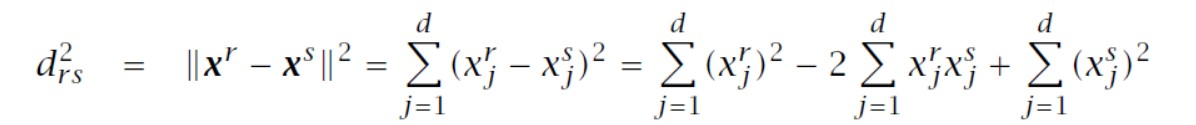
\includegraphics{image2.jpg}
\end{center}

    Now if we define \(b_{rs}\) as \[B = X*X^{T}\] or more precisely,
    \mbox{}
    \begin{center}
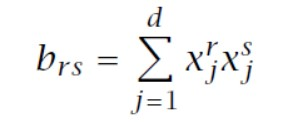
\includegraphics[scale = 0.6]{image.jpg}
\end{center}

    we get \(d^{2}_{rs}\) as,
    \mbox{}
    \begin{center}
    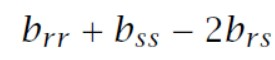
\includegraphics[scale = 0.6]{image1.jpg}
    \end{center}

    Note that this is zero mean. The sum of all data points will be equal to
zero. This is a constraint on the data

    Using the matrix B, we can get the eigen vectors of B and then the eigen
values from those vectors. We choose \(k\) dimensions, where,
\(k < min (d , N)\)

    Multi-dimensional scaling does the same thing as PCA, 1. Both have a
linear relationship with the original dimension \(d\) 2. PCA is
calculated on Covariance matrix, whereas MDS is calculated on
Correlation matrix. Essentially PCA on correlation matrix is the same as
MDS with euclildean distance with unit variance variables. 3. PCA does
this more efficiently

    The objectives in brief can be written as : 1. As an exploratory
technique to identify unrecognized dimensions affecting behavior 2. As a
means of obtaining comparative evaluations of objects when the specific
bases of comparison are unknown or undefinable

    \hypertarget{principal-component-analysis-pca-and-linear-discriminant-analysis-lda}{%
\section{Principal Component Analysis (PCA) and Linear Discriminant
Analysis
(LDA)}\label{principal-component-analysis-pca-and-linear-discriminant-analysis-lda}}

    \hypertarget{principal-component-analysis}{%
\subsection{Principal component
Analysis}\label{principal-component-analysis}}

    In projection methods we try to find the mapping of input space in \(d\)
dimensions to a new \(k ( < d)\) dimensions, with minimum loss of
information. The projection of x on the direction w is, \[Z = W^{T}*X\]

    PCA is an unsupervised dimensionality reduction method (Does not require
targets). It aims to find the principal component \(w\) of \(x\) such
that \(w\) has maximum variance (The difference between different points
is maximum). To ensure solution is unique \(||w||\) is equal to 1, this
also makes the direction important.

    Consider, \[Var(Z) = W^{T}*X\] PCA aims to maximize \(Var(Z)\) and keep
\(||W|| = 1\)

    Additionally the second principal component has to be orthogonal to the
previous principal component (Dot product is zero). This ensures the
correlation is minimized. In brief: 1. PCA is an unsupervised
algorithm(Requires no targets) 2. PCA uses the covariance matrix to find
projection onto the new dimensions. 3. PCA maximizes varaince in the
data and reduces correlation 4. The eigen values are calculated using
eigen vectors and these are arranged in descending order. The first
principal component contributes the maximum variance and so on.

    \hypertarget{linear-discriminant-analysis}{%
\subsection{Linear discriminant
analysis}\label{linear-discriminant-analysis}}

    Linear discriminant analysis is a supervised technique(Requires targets)
for dimensionality reduction, mainly used for classification. Given
samples from classes C1 and C2, LDA finds a projection from the original
\(d\) dimension to \(k < min ( d , n)\) dimensions such that the
seperation between the two classes is maximum. Here \(n\) is the number
of classes

    LDA is also called Fisher's linear discriminant. The objective function
is called Fisher's criterion J(w). The Fisher criterion is defined to be
the ratio of the between-class variance to the within-class variance.

    LDA also finds a projection of the data (Like PCA) but also uses the
targets to maximise the distance between classes (Unlike PCA)

    The projection is given by, \[Z = W^{T}*X\]

    While also optimizing the Fisher's Criterion \(J(W)\) given by,
\[J(W) = \frac{(m_{1} - m_{2})^{2}}{(s_{1}^{2}+s_{2}^{2})}\] where,
\(m_{i}\) is the mean of the class \(i\) \(s_{i}^{2}\) is the scatter
(Within class) of class \(i\)

    LDA essentially increase the distance between the means of the classes
while at the same time decreasing the within class scatter of the class.
This is encapsulated by th Fisher's Criterion

    In brief: 1. LDA is a dimnesionality reduction method that is supervised
(Requires targets) 2. LDA is also a classifier of sorts. It aims for
maximum seperation 3. Uses covariance matrix to find projection. And
hence the number of samples has to be big (Otherwise inversion gives a
singular value) 4. The resultant features are arranged in descending
order of the seperation contribution. The first feature seperates the
the most and so on.

    \hypertarget{demonstration-of-dimensionality-reduction}{%
\section{Demonstration of Dimensionality
Reduction}\label{demonstration-of-dimensionality-reduction}}

    \hypertarget{imporing-necessary-libraries}{%
\subsection{Imporing necessary
libraries}\label{imporing-necessary-libraries}}

    \begin{tcolorbox}[breakable, size=fbox, boxrule=1pt, pad at break*=1mm,colback=cellbackground, colframe=cellborder]
\prompt{In}{incolor}{93}{\boxspacing}
\begin{Verbatim}[commandchars=\\\{\}]
\PY{k+kn}{import} \PY{n+nn}{numpy} \PY{k}{as} \PY{n+nn}{np}
\PY{k+kn}{import} \PY{n+nn}{pandas} \PY{k}{as} \PY{n+nn}{pd}
\PY{k+kn}{import} \PY{n+nn}{matplotlib}\PY{n+nn}{.}\PY{n+nn}{pyplot} \PY{k}{as} \PY{n+nn}{plt}
\PY{k+kn}{import} \PY{n+nn}{seaborn} \PY{k}{as} \PY{n+nn}{sns}
\PY{k+kn}{from} \PY{n+nn}{sklearn}\PY{n+nn}{.}\PY{n+nn}{decomposition} \PY{k+kn}{import} \PY{n}{PCA}
\PY{k+kn}{from} \PY{n+nn}{sklearn}\PY{n+nn}{.}\PY{n+nn}{discriminant\PYZus{}analysis} \PY{k+kn}{import} \PY{n}{LinearDiscriminantAnalysis} \PY{k}{as} \PY{n}{LDA}
\PY{k+kn}{import} \PY{n+nn}{tensorflow} \PY{k}{as} \PY{n+nn}{tf}
\PY{k+kn}{from} \PY{n+nn}{sklearn}\PY{n+nn}{.}\PY{n+nn}{model\PYZus{}selection} \PY{k+kn}{import} \PY{n}{train\PYZus{}test\PYZus{}split}
\PY{k+kn}{from} \PY{n+nn}{mpl\PYZus{}toolkits}\PY{n+nn}{.}\PY{n+nn}{mplot3d} \PY{k+kn}{import} \PY{n}{Axes3D}
\end{Verbatim}
\end{tcolorbox}

    \hypertarget{get-the-data-from-here}{%
\subsubsection{Get the data from here:}\label{get-the-data-from-here}}

https://www.kaggle.com/dipayanbiswas/parkinsons-disease-speech-signal-features
The data consists of time series data of speech features of people
suffering from parkinsons disease. There are originally 750 features, of
which , 300 have been selected. The status of the person is the target
variable.

    \begin{tcolorbox}[breakable, size=fbox, boxrule=1pt, pad at break*=1mm,colback=cellbackground, colframe=cellborder]
\prompt{In}{incolor}{17}{\boxspacing}
\begin{Verbatim}[commandchars=\\\{\}]
\PY{n}{data} \PY{o}{=} \PY{n}{pd}\PY{o}{.}\PY{n}{read\PYZus{}csv}\PY{p}{(}\PY{l+s+s2}{\PYZdq{}}\PY{l+s+s2}{../Datasets/pd\PYZus{}speech\PYZus{}features.csv}\PY{l+s+s2}{\PYZdq{}}\PY{p}{)}
\PY{n}{data} \PY{o}{=} \PY{n}{data}\PY{o}{.}\PY{n}{drop}\PY{p}{(}\PY{n}{data}\PY{o}{.}\PY{n}{columns}\PY{p}{[}\PY{l+m+mi}{300}\PY{p}{:}\PY{o}{\PYZhy{}}\PY{l+m+mi}{1}\PY{p}{]}\PY{p}{,}\PY{n}{axis} \PY{o}{=} \PY{l+m+mi}{1}\PY{p}{)}
\PY{n}{data} \PY{o}{=} \PY{n}{data}\PY{o}{.}\PY{n}{drop}\PY{p}{(}\PY{l+s+s2}{\PYZdq{}}\PY{l+s+s2}{id}\PY{l+s+s2}{\PYZdq{}}\PY{p}{,}\PY{n}{axis} \PY{o}{=} \PY{l+m+mi}{1}\PY{p}{)}
\end{Verbatim}
\end{tcolorbox}

    \hypertarget{view-data-samples}{%
\subsection{View data samples}\label{view-data-samples}}

    \begin{tcolorbox}[breakable, size=fbox, boxrule=1pt, pad at break*=1mm,colback=cellbackground, colframe=cellborder]
\prompt{In}{incolor}{18}{\boxspacing}
\begin{Verbatim}[commandchars=\\\{\}]
\PY{n}{data}\PY{o}{.}\PY{n}{head}\PY{p}{(}\PY{p}{)}
\end{Verbatim}
\end{tcolorbox}

            \begin{tcolorbox}[breakable, size=fbox, boxrule=.5pt, pad at break*=1mm, opacityfill=0]
\prompt{Out}{outcolor}{18}{\boxspacing}
\begin{Verbatim}[commandchars=\\\{\}]
   gender      PPE      DFA     RPDE  numPulses  numPeriodsPulses  \textbackslash{}
0       1  0.85247  0.71826  0.57227        240               239
1       1  0.76686  0.69481  0.53966        234               233
2       1  0.85083  0.67604  0.58982        232               231
3       0  0.41121  0.79672  0.59257        178               177
4       0  0.32790  0.79782  0.53028        236               235

   meanPeriodPulses  stdDevPeriodPulses  locPctJitter  locAbsJitter  {\ldots}  \textbackslash{}
0          0.008064            0.000087       0.00218      0.000018  {\ldots}
1          0.008258            0.000073       0.00195      0.000016  {\ldots}
2          0.008340            0.000060       0.00176      0.000015  {\ldots}
3          0.010858            0.000183       0.00419      0.000046  {\ldots}
4          0.008162            0.002669       0.00535      0.000044  {\ldots}

   app\_LT\_entropy\_shannon\_10\_coef  app\_LT\_entropy\_log\_1\_coef  \textbackslash{}
0                    -3601122.613                   414.6434
1                    -3563560.603                   413.5284
2                    -3539902.400                   413.0675
3                    -3271399.011                   413.6380
4                    -3367165.736                   421.1396

   app\_LT\_entropy\_log\_2\_coef  app\_LT\_entropy\_log\_3\_coef  \textbackslash{}
0                   276.4850                   198.5803
1                   275.8597                   198.1971
2                   275.5868                   198.0149
3                   275.3259                   197.2795
4                   279.1703                   199.4350

   app\_LT\_entropy\_log\_4\_coef  app\_LT\_entropy\_log\_5\_coef  \textbackslash{}
0                   153.8978                   132.2489
1                   153.6379                   132.0522
2                   153.5036                   131.9418
3                   152.5940                   130.9480
4                   153.7788                   131.6258

   app\_LT\_entropy\_log\_6\_coef  app\_LT\_entropy\_log\_7\_coef  \textbackslash{}
0                   124.1971                   127.9812
1                   124.0327                   127.8282
2                   123.9329                   127.7329
3                   122.8786                   126.6411
4                   123.3566                   127.0837

   app\_LT\_entropy\_log\_8\_coef  class
0                   130.3804      1
1                   130.2373      1
2                   130.1464      1
3                   129.0689      1
4                   129.4029      1

[5 rows x 300 columns]
\end{Verbatim}
\end{tcolorbox}
        
    \hypertarget{checking-data-dimensions}{%
\subsection{Checking data dimensions}\label{checking-data-dimensions}}

    \begin{tcolorbox}[breakable, size=fbox, boxrule=1pt, pad at break*=1mm,colback=cellbackground, colframe=cellborder]
\prompt{In}{incolor}{19}{\boxspacing}
\begin{Verbatim}[commandchars=\\\{\}]
\PY{n}{data}\PY{o}{.}\PY{n}{shape}
\end{Verbatim}
\end{tcolorbox}

            \begin{tcolorbox}[breakable, size=fbox, boxrule=.5pt, pad at break*=1mm, opacityfill=0]
\prompt{Out}{outcolor}{19}{\boxspacing}
\begin{Verbatim}[commandchars=\\\{\}]
(756, 300)
\end{Verbatim}
\end{tcolorbox}
        
    \hypertarget{exploring-statistical-moments-of-the-data}{%
\subsection{Exploring statistical moments of the
data}\label{exploring-statistical-moments-of-the-data}}

At first glance it is clear that we need to normalize the data as the
mean of different attributes is different. From the features itself we
can see that they are on different scales (Exponential,logarithmic)
because of the feature extraction.

    \begin{tcolorbox}[breakable, size=fbox, boxrule=1pt, pad at break*=1mm,colback=cellbackground, colframe=cellborder]
\prompt{In}{incolor}{20}{\boxspacing}
\begin{Verbatim}[commandchars=\\\{\}]
\PY{n}{data}\PY{o}{.}\PY{n}{describe}\PY{p}{(}\PY{p}{)}
\end{Verbatim}
\end{tcolorbox}

            \begin{tcolorbox}[breakable, size=fbox, boxrule=.5pt, pad at break*=1mm, opacityfill=0]
\prompt{Out}{outcolor}{20}{\boxspacing}
\begin{Verbatim}[commandchars=\\\{\}]
           gender         PPE         DFA        RPDE   numPulses  \textbackslash{}
count  756.000000  756.000000  756.000000  756.000000  756.000000
mean     0.515873    0.746284    0.700414    0.489058  323.972222
std      0.500079    0.169294    0.069718    0.137442   99.219059
min      0.000000    0.041551    0.543500    0.154300    2.000000
25\%      0.000000    0.762833    0.647053    0.386537  251.000000
50\%      1.000000    0.809655    0.700525    0.484355  317.000000
75\%      1.000000    0.834315    0.754985    0.586515  384.250000
max      1.000000    0.907660    0.852640    0.871230  907.000000

       numPeriodsPulses  meanPeriodPulses  stdDevPeriodPulses  locPctJitter  \textbackslash{}
count        756.000000        756.000000          756.000000    756.000000
mean         322.678571          0.006360            0.000383      0.002324
std           99.402499          0.001826            0.000728      0.002628
min            1.000000          0.002107            0.000011      0.000210
25\%          250.000000          0.005003            0.000049      0.000970
50\%          316.000000          0.006048            0.000077      0.001495
75\%          383.250000          0.007528            0.000171      0.002520
max          905.000000          0.012966            0.003483      0.027750

       locAbsJitter  {\ldots}  app\_LT\_entropy\_shannon\_10\_coef  \textbackslash{}
count  7.560000e+02  {\ldots}                    7.560000e+02
mean   1.673391e-05  {\ldots}                   -4.143375e+06
std    2.290134e-05  {\ldots}                    4.876751e+05
min    6.860000e-07  {\ldots}                   -5.882489e+06
25\%    5.260000e-06  {\ldots}                   -4.474741e+06
50\%    9.530000e-06  {\ldots}                   -4.155440e+06
75\%    1.832500e-05  {\ldots}                   -3.802516e+06
max    2.564800e-04  {\ldots}                   -2.665481e+06

       app\_LT\_entropy\_log\_1\_coef  app\_LT\_entropy\_log\_2\_coef  \textbackslash{}
count                 756.000000                 756.000000
mean                  425.629078                 282.711578
std                    22.146419                  12.763780
min                   138.297600                 115.908600
25\%                   419.073075                 279.039500
50\%                   428.110650                 284.092300
75\%                   435.746200                 288.434200
max                   467.377300                 305.941900

       app\_LT\_entropy\_log\_3\_coef  app\_LT\_entropy\_log\_4\_coef  \textbackslash{}
count                 756.000000                 756.000000
mean                  202.511481                 156.685856
std                     7.567502                   4.475900
min                   106.489700                 102.332000
25\%                   200.170825                 155.049100
50\%                   203.374950                 157.179700
75\%                   206.039200                 159.002800
max                   216.634100                 166.016500

       app\_LT\_entropy\_log\_5\_coef  app\_LT\_entropy\_log\_6\_coef  \textbackslash{}
count                 756.000000                 756.000000
mean                  134.482587                 126.164411
std                     2.819619                   2.067284
min                   107.374200                 111.134600
25\%                   133.138125                 124.978700
50\%                   134.804800                 126.390950
75\%                   136.164075                 127.547025
max                   141.399600                 131.865800

       app\_LT\_entropy\_log\_7\_coef  app\_LT\_entropy\_log\_8\_coef       class
count                 756.000000                 756.000000  756.000000
mean                  129.842591                 132.197901    0.746032
std                     1.888099                   1.632429    0.435568
min                   121.331100                 126.152000    0.000000
25\%                   128.718000                 131.123125    0.000000
50\%                   130.046450                 132.335200    1.000000
75\%                   131.134600                 133.346950    1.000000
max                   135.165000                 137.089700    1.000000

[8 rows x 300 columns]
\end{Verbatim}
\end{tcolorbox}
        
    \hypertarget{exploring-the-distribution-of-classes}{%
\subsection{Exploring the distribution of
classes}\label{exploring-the-distribution-of-classes}}

The class distribution is skewed. From this skewed data we derive the
baseline accuracy which is 74\%. If the classifier acts like a majority
classifier (Outputs a constant value) it will have 74\% accuracy. For
our model to make a difference we need to exceed this at the least.

    \begin{tcolorbox}[breakable, size=fbox, boxrule=1pt, pad at break*=1mm,colback=cellbackground, colframe=cellborder]
\prompt{In}{incolor}{22}{\boxspacing}
\begin{Verbatim}[commandchars=\\\{\}]
\PY{n}{target} \PY{o}{=} \PY{n}{data}\PY{p}{[}\PY{l+s+s2}{\PYZdq{}}\PY{l+s+s2}{class}\PY{l+s+s2}{\PYZdq{}}\PY{p}{]}
\PY{n}{data\PYZus{}sec} \PY{o}{=} \PY{n}{data}\PY{p}{[}\PY{n}{data}\PY{o}{.}\PY{n}{columns}\PY{p}{[}\PY{p}{:}\PY{o}{\PYZhy{}}\PY{l+m+mi}{1}\PY{p}{]}\PY{p}{]}
\end{Verbatim}
\end{tcolorbox}

    \begin{tcolorbox}[breakable, size=fbox, boxrule=1pt, pad at break*=1mm,colback=cellbackground, colframe=cellborder]
\prompt{In}{incolor}{38}{\boxspacing}
\begin{Verbatim}[commandchars=\\\{\}]
\PY{n}{sns}\PY{o}{.}\PY{n}{countplot}\PY{p}{(}\PY{n}{target}\PY{p}{)}
\PY{n+nb}{print}\PY{p}{(}\PY{n}{target}\PY{o}{.}\PY{n}{value\PYZus{}counts}\PY{p}{(}\PY{p}{)}\PY{p}{)}
\PY{n+nb}{print}\PY{p}{(}\PY{l+s+s2}{\PYZdq{}}\PY{l+s+s2}{Baseline}\PY{l+s+s2}{\PYZdq{}}\PY{p}{,}\PY{p}{(}\PY{n}{target}\PY{o}{.}\PY{n}{value\PYZus{}counts}\PY{p}{(}\PY{p}{)}\PY{p}{[}\PY{l+m+mi}{1}\PY{p}{]}\PY{o}{/}\PY{n}{target}\PY{o}{.}\PY{n}{shape}\PY{p}{[}\PY{l+m+mi}{0}\PY{p}{]}\PY{p}{)}\PY{o}{*}\PY{l+m+mi}{100}\PY{p}{,}\PY{l+s+s2}{\PYZdq{}}\PY{l+s+s2}{\PYZpc{}}\PY{l+s+s2}{\PYZdq{}}\PY{p}{)}
\end{Verbatim}
\end{tcolorbox}

    \begin{Verbatim}[commandchars=\\\{\}]
1    564
0    192
Name: class, dtype: int64
Baseline 74.60317460317461 \%
    \end{Verbatim}

    \begin{center}
    \adjustimage{max size={0.9\linewidth}{0.9\paperheight}}{output_40_1.png}
    \end{center}
    { \hspace*{\fill} \\}
    
    \hypertarget{train-test-split}{%
\subsection{Train-Test split}\label{train-test-split}}

The post distribution is printed later The data is also normalized.

    \begin{tcolorbox}[breakable, size=fbox, boxrule=1pt, pad at break*=1mm,colback=cellbackground, colframe=cellborder]
\prompt{In}{incolor}{145}{\boxspacing}
\begin{Verbatim}[commandchars=\\\{\}]
\PY{n}{X\PYZus{}train}\PY{p}{,}\PY{n}{X\PYZus{}test}\PY{p}{,}\PY{n}{Y\PYZus{}train}\PY{p}{,}\PY{n}{Y\PYZus{}test} \PY{o}{=} \PY{n}{train\PYZus{}test\PYZus{}split}\PY{p}{(}\PY{n}{data\PYZus{}sec}\PY{p}{,}\PY{n}{target}\PY{p}{,}\PY{n}{test\PYZus{}size} \PY{o}{=} \PY{l+m+mf}{0.2}\PY{p}{)}
\end{Verbatim}
\end{tcolorbox}

    \begin{tcolorbox}[breakable, size=fbox, boxrule=1pt, pad at break*=1mm,colback=cellbackground, colframe=cellborder]
\prompt{In}{incolor}{146}{\boxspacing}
\begin{Verbatim}[commandchars=\\\{\}]
\PY{n+nb}{print}\PY{p}{(}\PY{n}{X\PYZus{}train}\PY{o}{.}\PY{n}{shape}\PY{p}{,}\PY{n}{Y\PYZus{}train}\PY{o}{.}\PY{n}{shape}\PY{p}{)}
\PY{n+nb}{print}\PY{p}{(}\PY{n}{X\PYZus{}test}\PY{o}{.}\PY{n}{shape}\PY{p}{,}\PY{n}{Y\PYZus{}test}\PY{o}{.}\PY{n}{shape}\PY{p}{)}
\end{Verbatim}
\end{tcolorbox}

    \begin{Verbatim}[commandchars=\\\{\}]
(604, 299) (604,)
(152, 299) (152,)
    \end{Verbatim}

    \begin{tcolorbox}[breakable, size=fbox, boxrule=1pt, pad at break*=1mm,colback=cellbackground, colframe=cellborder]
\prompt{In}{incolor}{147}{\boxspacing}
\begin{Verbatim}[commandchars=\\\{\}]
\PY{n}{X\PYZus{}train} \PY{o}{=} \PY{p}{(}\PY{n}{X\PYZus{}train} \PY{o}{\PYZhy{}} \PY{n}{X\PYZus{}train}\PY{o}{.}\PY{n}{mean}\PY{p}{(}\PY{p}{)}\PY{p}{)}\PY{o}{/}\PY{n}{X\PYZus{}train}\PY{o}{.}\PY{n}{std}\PY{p}{(}\PY{p}{)}
\PY{n}{X\PYZus{}test} \PY{o}{=} \PY{p}{(}\PY{n}{X\PYZus{}test} \PY{o}{\PYZhy{}} \PY{n}{X\PYZus{}test}\PY{o}{.}\PY{n}{mean}\PY{p}{(}\PY{p}{)}\PY{p}{)}\PY{o}{/}\PY{n}{X\PYZus{}test}\PY{o}{.}\PY{n}{std}\PY{p}{(}\PY{p}{)}
\end{Verbatim}
\end{tcolorbox}

    \hypertarget{applying-pca-on-the-data}{%
\subsection{Applying PCA on the data}\label{applying-pca-on-the-data}}

We plot the explained variance ratio vs the number of features to see
how many features explain the overall variance. Recall, PCA aims to
maximise variance in its principal components

    \begin{tcolorbox}[breakable, size=fbox, boxrule=1pt, pad at break*=1mm,colback=cellbackground, colframe=cellborder]
\prompt{In}{incolor}{149}{\boxspacing}
\begin{Verbatim}[commandchars=\\\{\}]
\PY{n}{pca} \PY{o}{=} \PY{n}{PCA}\PY{p}{(}\PY{p}{)}\PY{o}{.}\PY{n}{fit}\PY{p}{(}\PY{n}{X\PYZus{}train}\PY{p}{)}
\PY{n}{X\PYZus{}pca} \PY{o}{=} \PY{n}{pca}\PY{o}{.}\PY{n}{fit\PYZus{}transform}\PY{p}{(}\PY{n}{X\PYZus{}train}\PY{p}{)}
\PY{n}{X\PYZus{}pca\PYZus{}test} \PY{o}{=} \PY{n}{pca}\PY{o}{.}\PY{n}{fit\PYZus{}transform}\PY{p}{(}\PY{n}{X\PYZus{}test}\PY{p}{)}
\PY{n}{sums} \PY{o}{=} \PY{n}{np}\PY{o}{.}\PY{n}{cumsum}\PY{p}{(}\PY{n}{pca}\PY{o}{.}\PY{n}{explained\PYZus{}variance\PYZus{}ratio\PYZus{}}\PY{p}{)}
\PY{n}{plt}\PY{o}{.}\PY{n}{plot}\PY{p}{(}\PY{n}{np}\PY{o}{.}\PY{n}{cumsum}\PY{p}{(}\PY{n}{pca}\PY{o}{.}\PY{n}{explained\PYZus{}variance\PYZus{}ratio\PYZus{}}\PY{p}{)}\PY{p}{)}
\PY{n}{plt}\PY{o}{.}\PY{n}{xlabel}\PY{p}{(}\PY{l+s+s2}{\PYZdq{}}\PY{l+s+s2}{Number of Components}\PY{l+s+s2}{\PYZdq{}}\PY{p}{)}
\PY{n}{plt}\PY{o}{.}\PY{n}{ylabel}\PY{p}{(}\PY{l+s+s2}{\PYZdq{}}\PY{l+s+s2}{Explained Variance ratio}\PY{l+s+s2}{\PYZdq{}}\PY{p}{)}
\end{Verbatim}
\end{tcolorbox}

            \begin{tcolorbox}[breakable, size=fbox, boxrule=.5pt, pad at break*=1mm, opacityfill=0]
\prompt{Out}{outcolor}{149}{\boxspacing}
\begin{Verbatim}[commandchars=\\\{\}]
Text(0, 0.5, 'Explained Variance ratio')
\end{Verbatim}
\end{tcolorbox}
        
    \begin{center}
    \adjustimage{max size={0.9\linewidth}{0.9\paperheight}}{output_46_1.png}
    \end{center}
    { \hspace*{\fill} \\}
    
    \begin{tcolorbox}[breakable, size=fbox, boxrule=1pt, pad at break*=1mm,colback=cellbackground, colframe=cellborder]
\prompt{In}{incolor}{72}{\boxspacing}
\begin{Verbatim}[commandchars=\\\{\}]
\PY{n}{sums}\PY{p}{[}\PY{l+m+mi}{80}\PY{p}{]}
\end{Verbatim}
\end{tcolorbox}

            \begin{tcolorbox}[breakable, size=fbox, boxrule=.5pt, pad at break*=1mm, opacityfill=0]
\prompt{Out}{outcolor}{72}{\boxspacing}
\begin{Verbatim}[commandchars=\\\{\}]
0.9657289439379847
\end{Verbatim}
\end{tcolorbox}
        
    \hypertarget{visualization-of-pca-components.}{%
\subsection{Visualization of PCA
components.}\label{visualization-of-pca-components.}}

The original data with 300 features cannot be visualized but using PCA,
most of the variance can be visualized.

    \begin{tcolorbox}[breakable, size=fbox, boxrule=1pt, pad at break*=1mm,colback=cellbackground, colframe=cellborder]
\prompt{In}{incolor}{91}{\boxspacing}
\begin{Verbatim}[commandchars=\\\{\}]
\PY{n}{sns}\PY{o}{.}\PY{n}{scatterplot}\PY{p}{(}\PY{n}{X\PYZus{}pca}\PY{p}{[}\PY{p}{:}\PY{p}{,}\PY{l+m+mi}{0}\PY{p}{]}\PY{p}{,}\PY{n}{X\PYZus{}pca}\PY{p}{[}\PY{p}{:}\PY{p}{,}\PY{l+m+mi}{1}\PY{p}{]}\PY{p}{,}\PY{n}{hue} \PY{o}{=} \PY{n}{Y\PYZus{}train}\PY{p}{)}
\PY{n}{plt}\PY{o}{.}\PY{n}{xlabel}\PY{p}{(}\PY{l+s+s2}{\PYZdq{}}\PY{l+s+s2}{PCA Component 1}\PY{l+s+s2}{\PYZdq{}}\PY{p}{)}
\PY{n}{plt}\PY{o}{.}\PY{n}{ylabel}\PY{p}{(}\PY{l+s+s2}{\PYZdq{}}\PY{l+s+s2}{PCA Component 2}\PY{l+s+s2}{\PYZdq{}}\PY{p}{)}
\end{Verbatim}
\end{tcolorbox}

            \begin{tcolorbox}[breakable, size=fbox, boxrule=.5pt, pad at break*=1mm, opacityfill=0]
\prompt{Out}{outcolor}{91}{\boxspacing}
\begin{Verbatim}[commandchars=\\\{\}]
Text(0, 0.5, 'PCA Component 2')
\end{Verbatim}
\end{tcolorbox}
        
    \begin{center}
    \adjustimage{max size={0.9\linewidth}{0.9\paperheight}}{output_49_1.png}
    \end{center}
    { \hspace*{\fill} \\}
    
    \hypertarget{dimensional-visualization}{%
\subsubsection{3-Dimensional
visualization}\label{dimensional-visualization}}

As we see from both visualizations, the varianca is maximized, the
seperation is not so good. PCA is unsupervised and is not even trying to
seperate.

    \begin{tcolorbox}[breakable, size=fbox, boxrule=1pt, pad at break*=1mm,colback=cellbackground, colframe=cellborder]
\prompt{In}{incolor}{102}{\boxspacing}
\begin{Verbatim}[commandchars=\\\{\}]
\PY{n}{ax} \PY{o}{=} \PY{n}{Axes3D}\PY{p}{(}\PY{n}{plt}\PY{o}{.}\PY{n}{figure}\PY{p}{(}\PY{p}{)}\PY{p}{)}
\PY{n}{p} \PY{o}{=} \PY{n}{ax}\PY{o}{.}\PY{n}{scatter}\PY{p}{(}\PY{n}{X\PYZus{}pca}\PY{p}{[}\PY{p}{:}\PY{p}{,} \PY{l+m+mi}{0}\PY{p}{]}\PY{p}{,} \PY{n}{X\PYZus{}pca}\PY{p}{[}\PY{p}{:}\PY{p}{,} \PY{l+m+mi}{1}\PY{p}{]}\PY{p}{,}\PY{n}{X\PYZus{}pca}\PY{p}{[}\PY{p}{:}\PY{p}{,}\PY{l+m+mi}{2}\PY{p}{]}\PY{p}{,}
            \PY{n}{c}\PY{o}{=}\PY{n}{Y\PYZus{}train}\PY{p}{,} \PY{n}{alpha}\PY{o}{=}\PY{l+m+mf}{0.5}\PY{p}{,}
            \PY{n}{cmap}\PY{o}{=}\PY{n}{plt}\PY{o}{.}\PY{n}{cm}\PY{o}{.}\PY{n}{get\PYZus{}cmap}\PY{p}{(}\PY{l+s+s1}{\PYZsq{}}\PY{l+s+s1}{vlag\PYZus{}r}\PY{l+s+s1}{\PYZsq{}}\PY{p}{,} \PY{l+m+mi}{2}\PY{p}{)}\PY{p}{)}
\PY{n}{plt}\PY{o}{.}\PY{n}{xlabel}\PY{p}{(}\PY{l+s+s1}{\PYZsq{}}\PY{l+s+s1}{component 1}\PY{l+s+s1}{\PYZsq{}}\PY{p}{)}
\PY{n}{plt}\PY{o}{.}\PY{n}{ylabel}\PY{p}{(}\PY{l+s+s1}{\PYZsq{}}\PY{l+s+s1}{component 2}\PY{l+s+s1}{\PYZsq{}}\PY{p}{)}
\PY{n}{ax}\PY{o}{.}\PY{n}{set\PYZus{}zlabel}\PY{p}{(}\PY{l+s+s1}{\PYZsq{}}\PY{l+s+s1}{component 3}\PY{l+s+s1}{\PYZsq{}}\PY{p}{)}
\PY{n}{plt}\PY{o}{.}\PY{n}{colorbar}\PY{p}{(}\PY{n}{p}\PY{p}{)}\PY{p}{;}
\end{Verbatim}
\end{tcolorbox}

    \begin{center}
    \adjustimage{max size={0.9\linewidth}{0.9\paperheight}}{output_51_0.png}
    \end{center}
    { \hspace*{\fill} \\}
    
    \hypertarget{applying-lda-on-the-dataset}{%
\subsection{Applying LDA on the
dataset}\label{applying-lda-on-the-dataset}}

LDA features have to be less than
\(min ( number of samples, number of classes)\). Becuase number of
classes is 2, we obtain only one LDA feature. But this feature maximizes
the seperation. As we can see from the below plot. It is mostly
seperated using one dimension.

    \begin{tcolorbox}[breakable, size=fbox, boxrule=1pt, pad at break*=1mm,colback=cellbackground, colframe=cellborder]
\prompt{In}{incolor}{198}{\boxspacing}
\begin{Verbatim}[commandchars=\\\{\}]
\PY{n}{lda} \PY{o}{=} \PY{n}{LDA}\PY{p}{(}\PY{p}{)}\PY{o}{.}\PY{n}{fit\PYZus{}transform}\PY{p}{(}\PY{n}{X\PYZus{}train}\PY{p}{,}\PY{n}{Y\PYZus{}train}\PY{p}{)}
\PY{n}{lda\PYZus{}test} \PY{o}{=} \PY{n}{LDA}\PY{p}{(}\PY{p}{)}\PY{o}{.}\PY{n}{fit\PYZus{}transform}\PY{p}{(}\PY{n}{X\PYZus{}test}\PY{p}{,}\PY{n}{Y\PYZus{}test}\PY{p}{)}
\end{Verbatim}
\end{tcolorbox}

    \begin{tcolorbox}[breakable, size=fbox, boxrule=1pt, pad at break*=1mm,colback=cellbackground, colframe=cellborder]
\prompt{In}{incolor}{113}{\boxspacing}
\begin{Verbatim}[commandchars=\\\{\}]
\PY{n}{sns}\PY{o}{.}\PY{n}{scatterplot}\PY{p}{(}\PY{n}{lda}\PY{p}{[}\PY{p}{:}\PY{p}{,}\PY{l+m+mi}{0}\PY{p}{]}\PY{p}{,}\PY{l+m+mi}{1}\PY{p}{,}\PY{n}{hue} \PY{o}{=} \PY{n}{Y\PYZus{}train}\PY{p}{)}
\PY{n}{plt}\PY{o}{.}\PY{n}{xlabel}\PY{p}{(}\PY{l+s+s2}{\PYZdq{}}\PY{l+s+s2}{LDA Component 1}\PY{l+s+s2}{\PYZdq{}}\PY{p}{)}
\PY{n}{plt}\PY{o}{.}\PY{n}{ylabel}\PY{p}{(}\PY{l+s+s2}{\PYZdq{}}\PY{l+s+s2}{LDA Component 2}\PY{l+s+s2}{\PYZdq{}}\PY{p}{)}
\end{Verbatim}
\end{tcolorbox}

            \begin{tcolorbox}[breakable, size=fbox, boxrule=.5pt, pad at break*=1mm, opacityfill=0]
\prompt{Out}{outcolor}{113}{\boxspacing}
\begin{Verbatim}[commandchars=\\\{\}]
Text(0, 0.5, 'LDA Component 2')
\end{Verbatim}
\end{tcolorbox}
        
    \begin{center}
    \adjustimage{max size={0.9\linewidth}{0.9\paperheight}}{output_54_1.png}
    \end{center}
    { \hspace*{\fill} \\}
    
    \begin{tcolorbox}[breakable, size=fbox, boxrule=1pt, pad at break*=1mm,colback=cellbackground, colframe=cellborder]
\prompt{In}{incolor}{110}{\boxspacing}
\begin{Verbatim}[commandchars=\\\{\}]
\PY{n}{lda}\PY{o}{.}\PY{n}{shape}
\end{Verbatim}
\end{tcolorbox}

            \begin{tcolorbox}[breakable, size=fbox, boxrule=.5pt, pad at break*=1mm, opacityfill=0]
\prompt{Out}{outcolor}{110}{\boxspacing}
\begin{Verbatim}[commandchars=\\\{\}]
(604, 1)
\end{Verbatim}
\end{tcolorbox}
        
    \hypertarget{training-neural-net-on-original-data-features}{%
\subsection{Training Neural Net on original data
features}\label{training-neural-net-on-original-data-features}}

We get about 76.31\% on the test set. Which is above baseline.

    \begin{tcolorbox}[breakable, size=fbox, boxrule=1pt, pad at break*=1mm,colback=cellbackground, colframe=cellborder]
\prompt{In}{incolor}{141}{\boxspacing}
\begin{Verbatim}[commandchars=\\\{\}]
\PY{n}{model\PYZus{}orig} \PY{o}{=} \PY{n}{tf}\PY{o}{.}\PY{n}{keras}\PY{o}{.}\PY{n}{models}\PY{o}{.}\PY{n}{Sequential}\PY{p}{(}\PY{p}{[}\PY{n}{tf}\PY{o}{.}\PY{n}{keras}\PY{o}{.}\PY{n}{layers}\PY{o}{.}\PY{n}{Input}\PY{p}{(}\PY{l+m+mi}{299}\PY{p}{,}\PY{l+m+mi}{1}\PY{p}{)}\PY{p}{,}
                                        \PY{n}{tf}\PY{o}{.}\PY{n}{keras}\PY{o}{.}\PY{n}{layers}\PY{o}{.}\PY{n}{Dense}\PY{p}{(}\PY{n}{units} \PY{o}{=} \PY{l+m+mi}{256}\PY{p}{,}\PY{n}{activation} \PY{o}{=} \PY{n}{tf}\PY{o}{.}\PY{n}{nn}\PY{o}{.}\PY{n}{relu}\PY{p}{)}\PY{p}{,}
                                        \PY{n}{tf}\PY{o}{.}\PY{n}{keras}\PY{o}{.}\PY{n}{layers}\PY{o}{.}\PY{n}{Dense}\PY{p}{(}\PY{n}{units} \PY{o}{=} \PY{l+m+mi}{1}\PY{p}{,}\PY{n}{activation} \PY{o}{=} \PY{n}{tf}\PY{o}{.}\PY{n}{nn}\PY{o}{.}\PY{n}{sigmoid}\PY{p}{)}\PY{p}{]}\PY{p}{)}
\PY{n}{model\PYZus{}orig}\PY{o}{.}\PY{n}{compile}\PY{p}{(}\PY{n}{optimizer} \PY{o}{=} \PY{l+s+s2}{\PYZdq{}}\PY{l+s+s2}{adam}\PY{l+s+s2}{\PYZdq{}}\PY{p}{,}\PY{n}{loss} \PY{o}{=} \PY{l+s+s2}{\PYZdq{}}\PY{l+s+s2}{binary\PYZus{}crossentropy}\PY{l+s+s2}{\PYZdq{}}\PY{p}{,}\PY{n}{metrics} \PY{o}{=} \PY{p}{[}\PY{l+s+s2}{\PYZdq{}}\PY{l+s+s2}{accuracy}\PY{l+s+s2}{\PYZdq{}}\PY{p}{]}\PY{p}{)}
\PY{n}{model\PYZus{}orig}\PY{o}{.}\PY{n}{build}\PY{p}{(}\PY{p}{)}
\PY{n}{model\PYZus{}orig}\PY{o}{.}\PY{n}{summary}\PY{p}{(}\PY{p}{)}
\PY{n}{model\PYZus{}orig}\PY{o}{.}\PY{n}{fit}\PY{p}{(}\PY{n}{X\PYZus{}train}\PY{p}{,}\PY{n}{Y\PYZus{}train}\PY{o}{.}\PY{n}{values}\PY{p}{,}\PY{n}{epochs} \PY{o}{=} \PY{l+m+mi}{10}\PY{p}{)}
\end{Verbatim}
\end{tcolorbox}

    \begin{Verbatim}[commandchars=\\\{\}]
Model: "sequential\_7"
\_\_\_\_\_\_\_\_\_\_\_\_\_\_\_\_\_\_\_\_\_\_\_\_\_\_\_\_\_\_\_\_\_\_\_\_\_\_\_\_\_\_\_\_\_\_\_\_\_\_\_\_\_\_\_\_\_\_\_\_\_\_\_\_\_
Layer (type)                 Output Shape              Param \#
=================================================================
dense\_13 (Dense)             (1, 256)                  76800
\_\_\_\_\_\_\_\_\_\_\_\_\_\_\_\_\_\_\_\_\_\_\_\_\_\_\_\_\_\_\_\_\_\_\_\_\_\_\_\_\_\_\_\_\_\_\_\_\_\_\_\_\_\_\_\_\_\_\_\_\_\_\_\_\_
dense\_14 (Dense)             (1, 1)                    257
=================================================================
Total params: 77,057
Trainable params: 77,057
Non-trainable params: 0
\_\_\_\_\_\_\_\_\_\_\_\_\_\_\_\_\_\_\_\_\_\_\_\_\_\_\_\_\_\_\_\_\_\_\_\_\_\_\_\_\_\_\_\_\_\_\_\_\_\_\_\_\_\_\_\_\_\_\_\_\_\_\_\_\_
Epoch 1/10
604/604 [==============================] - 1s 2ms/sample - loss: 0.5901 - acc:
0.7715
Epoch 2/10
604/604 [==============================] - 1s 2ms/sample - loss: 0.2866 - acc:
0.8775
Epoch 3/10
604/604 [==============================] - 1s 2ms/sample - loss: 0.2381 - acc:
0.9023
Epoch 4/10
604/604 [==============================] - 1s 2ms/sample - loss: 0.1904 - acc:
0.9338
Epoch 5/10
604/604 [==============================] - 1s 2ms/sample - loss: 0.1586 - acc:
0.9487
Epoch 6/10
604/604 [==============================] - 1s 2ms/sample - loss: 0.1180 - acc:
0.9619
Epoch 7/10
604/604 [==============================] - 1s 2ms/sample - loss: 0.0598 - acc:
0.9834
Epoch 8/10
604/604 [==============================] - 1s 2ms/sample - loss: 0.0591 - acc:
0.9884
Epoch 9/10
604/604 [==============================] - 1s 2ms/sample - loss: 0.0573 - acc:
0.9818
Epoch 10/10
604/604 [==============================] - 1s 2ms/sample - loss: 0.0600 - acc:
0.9818
    \end{Verbatim}

            \begin{tcolorbox}[breakable, size=fbox, boxrule=.5pt, pad at break*=1mm, opacityfill=0]
\prompt{Out}{outcolor}{141}{\boxspacing}
\begin{Verbatim}[commandchars=\\\{\}]
<tensorflow.python.keras.callbacks.History at 0x1febb541888>
\end{Verbatim}
\end{tcolorbox}
        
    \begin{tcolorbox}[breakable, size=fbox, boxrule=1pt, pad at break*=1mm,colback=cellbackground, colframe=cellborder]
\prompt{In}{incolor}{144}{\boxspacing}
\begin{Verbatim}[commandchars=\\\{\}]
\PY{n+nb}{print}\PY{p}{(}\PY{n}{model\PYZus{}orig}\PY{o}{.}\PY{n}{evaluate}\PY{p}{(}\PY{n}{X\PYZus{}train}\PY{p}{,}\PY{n}{Y\PYZus{}train}\PY{o}{.}\PY{n}{values}\PY{p}{)}\PY{p}{[}\PY{l+m+mi}{1}\PY{p}{]}\PY{o}{*}\PY{l+m+mi}{100}\PY{p}{)}
\PY{n+nb}{print}\PY{p}{(}\PY{n}{model\PYZus{}orig}\PY{o}{.}\PY{n}{evaluate}\PY{p}{(}\PY{n}{X\PYZus{}test}\PY{p}{,}\PY{n}{Y\PYZus{}test}\PY{o}{.}\PY{n}{values}\PY{p}{)}\PY{p}{[}\PY{l+m+mi}{1}\PY{p}{]}\PY{o}{*}\PY{l+m+mi}{100}\PY{p}{)}
\end{Verbatim}
\end{tcolorbox}

    \begin{Verbatim}[commandchars=\\\{\}]
604/604 [==============================] - 1s 882us/sample - loss: 0.7026 - acc:
0.9255
92.54966974258423
152/152 [==============================] - 0s 886us/sample - loss: 1.3734 - acc:
0.7632
76.31579041481018
    \end{Verbatim}

    \hypertarget{training-neural-net-on-pca-features}{%
\subsection{Training Neural net on PCA
features}\label{training-neural-net-on-pca-features}}

We have taken the maximum amount of features, 150. We get about 76.9\%
test accuracy, which is pretty good. Although a good amount of
hyperpaprameter tuning was required

    \begin{tcolorbox}[breakable, size=fbox, boxrule=1pt, pad at break*=1mm,colback=cellbackground, colframe=cellborder]
\prompt{In}{incolor}{224}{\boxspacing}
\begin{Verbatim}[commandchars=\\\{\}]
\PY{n}{feat} \PY{o}{=} \PY{l+m+mi}{150}
\PY{n}{model\PYZus{}pca} \PY{o}{=} \PY{n}{tf}\PY{o}{.}\PY{n}{keras}\PY{o}{.}\PY{n}{models}\PY{o}{.}\PY{n}{Sequential}\PY{p}{(}\PY{p}{[}\PY{n}{tf}\PY{o}{.}\PY{n}{keras}\PY{o}{.}\PY{n}{layers}\PY{o}{.}\PY{n}{Input}\PY{p}{(}\PY{n}{feat}\PY{p}{,}\PY{l+m+mi}{1}\PY{p}{)}\PY{p}{,}
                                        \PY{n}{tf}\PY{o}{.}\PY{n}{keras}\PY{o}{.}\PY{n}{layers}\PY{o}{.}\PY{n}{Dense}\PY{p}{(}\PY{n}{units} \PY{o}{=} \PY{l+m+mi}{1024}\PY{p}{,}\PY{n}{activation} \PY{o}{=} \PY{n}{tf}\PY{o}{.}\PY{n}{nn}\PY{o}{.}\PY{n}{relu}\PY{p}{,}\PY{n}{kernel\PYZus{}regularizer} \PY{o}{=} \PY{n}{tf}\PY{o}{.}\PY{n}{keras}\PY{o}{.}\PY{n}{regularizers}\PY{o}{.}\PY{n}{l2}\PY{p}{(}\PY{l+m+mf}{0.7}\PY{p}{)}\PY{p}{)}\PY{p}{,}
                                        \PY{n}{tf}\PY{o}{.}\PY{n}{keras}\PY{o}{.}\PY{n}{layers}\PY{o}{.}\PY{n}{Dense}\PY{p}{(}\PY{n}{units} \PY{o}{=} \PY{l+m+mi}{1}\PY{p}{,}\PY{n}{activation} \PY{o}{=} \PY{n}{tf}\PY{o}{.}\PY{n}{nn}\PY{o}{.}\PY{n}{sigmoid}\PY{p}{)}\PY{p}{]}\PY{p}{)}
\PY{n}{model\PYZus{}pca}\PY{o}{.}\PY{n}{compile}\PY{p}{(}\PY{n}{optimizer} \PY{o}{=} \PY{l+s+s2}{\PYZdq{}}\PY{l+s+s2}{adam}\PY{l+s+s2}{\PYZdq{}}\PY{p}{,}\PY{n}{loss} \PY{o}{=} \PY{l+s+s2}{\PYZdq{}}\PY{l+s+s2}{binary\PYZus{}crossentropy}\PY{l+s+s2}{\PYZdq{}}\PY{p}{,}\PY{n}{metrics} \PY{o}{=} \PY{p}{[}\PY{l+s+s2}{\PYZdq{}}\PY{l+s+s2}{accuracy}\PY{l+s+s2}{\PYZdq{}}\PY{p}{]}\PY{p}{)}
\PY{n}{model\PYZus{}pca}\PY{o}{.}\PY{n}{build}\PY{p}{(}\PY{p}{)}
\PY{n}{model\PYZus{}pca}\PY{o}{.}\PY{n}{summary}\PY{p}{(}\PY{p}{)}
\PY{n}{model\PYZus{}pca}\PY{o}{.}\PY{n}{fit}\PY{p}{(}\PY{n}{X\PYZus{}pca}\PY{p}{[}\PY{p}{:}\PY{p}{,}\PY{p}{:}\PY{n}{feat}\PY{p}{]}\PY{p}{,}\PY{n}{Y\PYZus{}train}\PY{o}{.}\PY{n}{values}\PY{p}{,}\PY{n}{epochs} \PY{o}{=} \PY{l+m+mi}{20}\PY{p}{)}
\end{Verbatim}
\end{tcolorbox}

    \begin{Verbatim}[commandchars=\\\{\}]
Model: "sequential\_42"
\_\_\_\_\_\_\_\_\_\_\_\_\_\_\_\_\_\_\_\_\_\_\_\_\_\_\_\_\_\_\_\_\_\_\_\_\_\_\_\_\_\_\_\_\_\_\_\_\_\_\_\_\_\_\_\_\_\_\_\_\_\_\_\_\_
Layer (type)                 Output Shape              Param \#
=================================================================
dense\_83 (Dense)             (1, 1024)                 154624
\_\_\_\_\_\_\_\_\_\_\_\_\_\_\_\_\_\_\_\_\_\_\_\_\_\_\_\_\_\_\_\_\_\_\_\_\_\_\_\_\_\_\_\_\_\_\_\_\_\_\_\_\_\_\_\_\_\_\_\_\_\_\_\_\_
dense\_84 (Dense)             (1, 1)                    1025
=================================================================
Total params: 155,649
Trainable params: 155,649
Non-trainable params: 0
\_\_\_\_\_\_\_\_\_\_\_\_\_\_\_\_\_\_\_\_\_\_\_\_\_\_\_\_\_\_\_\_\_\_\_\_\_\_\_\_\_\_\_\_\_\_\_\_\_\_\_\_\_\_\_\_\_\_\_\_\_\_\_\_\_
Epoch 1/20
604/604 [==============================] - 2s 3ms/sample - loss: 7.3186 - acc:
0.7666
Epoch 2/20
604/604 [==============================] - 1s 2ms/sample - loss: 0.7312 - acc:
0.7748
Epoch 3/20
604/604 [==============================] - 1s 2ms/sample - loss: 0.7333 - acc:
0.7781
Epoch 4/20
604/604 [==============================] - 1s 2ms/sample - loss: 0.7175 - acc:
0.7765
Epoch 5/20
604/604 [==============================] - 1s 2ms/sample - loss: 0.6736 - acc:
0.7914
Epoch 6/20
604/604 [==============================] - 1s 2ms/sample - loss: 0.6500 - acc:
0.7781
Epoch 7/20
604/604 [==============================] - 1s 2ms/sample - loss: 0.6322 - acc:
0.7864
Epoch 8/20
604/604 [==============================] - 1s 2ms/sample - loss: 0.6201 - acc:
0.7964
Epoch 9/20
604/604 [==============================] - 1s 2ms/sample - loss: 0.5922 - acc:
0.8013
Epoch 10/20
604/604 [==============================] - 1s 2ms/sample - loss: 0.5757 - acc:
0.7930
Epoch 11/20
604/604 [==============================] - 1s 2ms/sample - loss: 0.5883 - acc:
0.7831
Epoch 12/20
604/604 [==============================] - 1s 2ms/sample - loss: 0.5669 - acc:
0.7864
Epoch 13/20
604/604 [==============================] - 1s 2ms/sample - loss: 0.5607 - acc:
0.7997
Epoch 14/20
604/604 [==============================] - 1s 2ms/sample - loss: 0.5600 - acc:
0.8013
Epoch 15/20
604/604 [==============================] - 1s 2ms/sample - loss: 0.5571 - acc:
0.7930
Epoch 16/20
604/604 [==============================] - 1s 2ms/sample - loss: 0.5412 - acc:
0.8063
Epoch 17/20
604/604 [==============================] - 1s 2ms/sample - loss: 0.5478 - acc:
0.8030
Epoch 18/20
604/604 [==============================] - 1s 2ms/sample - loss: 0.5466 - acc:
0.8046
Epoch 19/20
604/604 [==============================] - 1s 2ms/sample - loss: 0.5422 - acc:
0.7914
Epoch 20/20
604/604 [==============================] - 1s 2ms/sample - loss: 0.5381 - acc:
0.7980
    \end{Verbatim}

            \begin{tcolorbox}[breakable, size=fbox, boxrule=.5pt, pad at break*=1mm, opacityfill=0]
\prompt{Out}{outcolor}{224}{\boxspacing}
\begin{Verbatim}[commandchars=\\\{\}]
<tensorflow.python.keras.callbacks.History at 0x1ffa97f2488>
\end{Verbatim}
\end{tcolorbox}
        
    \begin{tcolorbox}[breakable, size=fbox, boxrule=1pt, pad at break*=1mm,colback=cellbackground, colframe=cellborder]
\prompt{In}{incolor}{225}{\boxspacing}
\begin{Verbatim}[commandchars=\\\{\}]
\PY{n+nb}{print}\PY{p}{(}\PY{n}{model\PYZus{}pca}\PY{o}{.}\PY{n}{evaluate}\PY{p}{(}\PY{n}{X\PYZus{}pca}\PY{p}{[}\PY{p}{:}\PY{p}{,}\PY{p}{:}\PY{n}{feat}\PY{p}{]}\PY{p}{,}\PY{n}{Y\PYZus{}train}\PY{o}{.}\PY{n}{values}\PY{p}{)}\PY{p}{[}\PY{l+m+mi}{1}\PY{p}{]}\PY{o}{*}\PY{l+m+mi}{100}\PY{p}{)}
\PY{n+nb}{print}\PY{p}{(}\PY{n}{model\PYZus{}pca}\PY{o}{.}\PY{n}{evaluate}\PY{p}{(}\PY{n}{X\PYZus{}pca\PYZus{}test}\PY{p}{[}\PY{p}{:}\PY{p}{,}\PY{p}{:}\PY{n}{feat}\PY{p}{]}\PY{p}{,}\PY{n}{Y\PYZus{}test}\PY{o}{.}\PY{n}{values}\PY{p}{)}\PY{p}{[}\PY{l+m+mi}{1}\PY{p}{]}\PY{o}{*}\PY{l+m+mi}{100}\PY{p}{)}
\end{Verbatim}
\end{tcolorbox}

    \begin{Verbatim}[commandchars=\\\{\}]
604/604 [==============================] - 1s 2ms/sample - loss: 0.4896 - acc:
0.8477
84.76821184158325
152/152 [==============================] - 0s 1ms/sample - loss: 0.7737 - acc:
0.7697
76.97368264198303
    \end{Verbatim}

    \hypertarget{training-a-neual-net-on-lda-feature-space}{%
\subsection{Training a Neual net on LDA feature
space}\label{training-a-neual-net-on-lda-feature-space}}

Recall, LDA aims to maximize seperation and this means that the job of
the classifier is made easier (Most times) We get a 100\% test accuracy.
Which is the best among all of the models.

    \begin{tcolorbox}[breakable, size=fbox, boxrule=1pt, pad at break*=1mm,colback=cellbackground, colframe=cellborder]
\prompt{In}{incolor}{199}{\boxspacing}
\begin{Verbatim}[commandchars=\\\{\}]
\PY{n}{feat} \PY{o}{=} \PY{l+m+mi}{1}
\PY{n}{model\PYZus{}lda} \PY{o}{=} \PY{n}{tf}\PY{o}{.}\PY{n}{keras}\PY{o}{.}\PY{n}{models}\PY{o}{.}\PY{n}{Sequential}\PY{p}{(}\PY{p}{[}\PY{n}{tf}\PY{o}{.}\PY{n}{keras}\PY{o}{.}\PY{n}{layers}\PY{o}{.}\PY{n}{Input}\PY{p}{(}\PY{n}{feat}\PY{p}{,}\PY{l+m+mi}{1}\PY{p}{)}\PY{p}{,}
                                        \PY{n}{tf}\PY{o}{.}\PY{n}{keras}\PY{o}{.}\PY{n}{layers}\PY{o}{.}\PY{n}{Dense}\PY{p}{(}\PY{n}{units} \PY{o}{=} \PY{l+m+mi}{256}\PY{p}{,}\PY{n}{activation} \PY{o}{=} \PY{n}{tf}\PY{o}{.}\PY{n}{nn}\PY{o}{.}\PY{n}{relu}\PY{p}{,}\PY{n}{kernel\PYZus{}regularizer} \PY{o}{=} \PY{n}{tf}\PY{o}{.}\PY{n}{keras}\PY{o}{.}\PY{n}{regularizers}\PY{o}{.}\PY{n}{l2}\PY{p}{(}\PY{l+m+mf}{0.01}\PY{p}{)}\PY{p}{)}\PY{p}{,}
                                        \PY{n}{tf}\PY{o}{.}\PY{n}{keras}\PY{o}{.}\PY{n}{layers}\PY{o}{.}\PY{n}{Dense}\PY{p}{(}\PY{n}{units} \PY{o}{=} \PY{l+m+mi}{1}\PY{p}{,}\PY{n}{activation} \PY{o}{=} \PY{n}{tf}\PY{o}{.}\PY{n}{nn}\PY{o}{.}\PY{n}{sigmoid}\PY{p}{)}\PY{p}{]}\PY{p}{)}
\PY{n}{model\PYZus{}lda}\PY{o}{.}\PY{n}{compile}\PY{p}{(}\PY{n}{optimizer} \PY{o}{=} \PY{l+s+s2}{\PYZdq{}}\PY{l+s+s2}{adam}\PY{l+s+s2}{\PYZdq{}}\PY{p}{,}\PY{n}{loss} \PY{o}{=} \PY{l+s+s2}{\PYZdq{}}\PY{l+s+s2}{binary\PYZus{}crossentropy}\PY{l+s+s2}{\PYZdq{}}\PY{p}{,}\PY{n}{metrics} \PY{o}{=} \PY{p}{[}\PY{l+s+s2}{\PYZdq{}}\PY{l+s+s2}{accuracy}\PY{l+s+s2}{\PYZdq{}}\PY{p}{]}\PY{p}{)}
\PY{n}{model\PYZus{}lda}\PY{o}{.}\PY{n}{build}\PY{p}{(}\PY{p}{)}
\PY{n}{model\PYZus{}lda}\PY{o}{.}\PY{n}{summary}\PY{p}{(}\PY{p}{)}
\PY{n}{model\PYZus{}lda}\PY{o}{.}\PY{n}{fit}\PY{p}{(}\PY{n}{lda}\PY{p}{[}\PY{p}{:}\PY{p}{,}\PY{p}{:}\PY{n}{feat}\PY{p}{]}\PY{p}{,}\PY{n}{Y\PYZus{}train}\PY{o}{.}\PY{n}{values}\PY{p}{,}\PY{n}{epochs} \PY{o}{=} \PY{l+m+mi}{10}\PY{p}{)}
\end{Verbatim}
\end{tcolorbox}

    \begin{Verbatim}[commandchars=\\\{\}]
Model: "sequential\_30"
\_\_\_\_\_\_\_\_\_\_\_\_\_\_\_\_\_\_\_\_\_\_\_\_\_\_\_\_\_\_\_\_\_\_\_\_\_\_\_\_\_\_\_\_\_\_\_\_\_\_\_\_\_\_\_\_\_\_\_\_\_\_\_\_\_
Layer (type)                 Output Shape              Param \#
=================================================================
dense\_59 (Dense)             (1, 256)                  512
\_\_\_\_\_\_\_\_\_\_\_\_\_\_\_\_\_\_\_\_\_\_\_\_\_\_\_\_\_\_\_\_\_\_\_\_\_\_\_\_\_\_\_\_\_\_\_\_\_\_\_\_\_\_\_\_\_\_\_\_\_\_\_\_\_
dense\_60 (Dense)             (1, 1)                    257
=================================================================
Total params: 769
Trainable params: 769
Non-trainable params: 0
\_\_\_\_\_\_\_\_\_\_\_\_\_\_\_\_\_\_\_\_\_\_\_\_\_\_\_\_\_\_\_\_\_\_\_\_\_\_\_\_\_\_\_\_\_\_\_\_\_\_\_\_\_\_\_\_\_\_\_\_\_\_\_\_\_
Epoch 1/10
604/604 [==============================] - 2s 3ms/sample - loss: 0.2425 - acc:
0.9139
Epoch 2/10
604/604 [==============================] - 1s 2ms/sample - loss: 0.1736 - acc:
0.9255
Epoch 3/10
604/604 [==============================] - 1s 2ms/sample - loss: 0.1689 - acc:
0.9288
Epoch 4/10
604/604 [==============================] - 1s 2ms/sample - loss: 0.1655 - acc:
0.9321
Epoch 5/10
604/604 [==============================] - 1s 2ms/sample - loss: 0.1660 - acc:
0.9305
Epoch 6/10
604/604 [==============================] - 1s 2ms/sample - loss: 0.1658 - acc:
0.9338
Epoch 7/10
604/604 [==============================] - 1s 2ms/sample - loss: 0.1645 - acc:
0.9321
Epoch 8/10
604/604 [==============================] - 1s 2ms/sample - loss: 0.1648 - acc:
0.9288
Epoch 9/10
604/604 [==============================] - 1s 2ms/sample - loss: 0.1650 - acc:
0.9288
Epoch 10/10
604/604 [==============================] - 1s 2ms/sample - loss: 0.1671 - acc:
0.9272
    \end{Verbatim}

            \begin{tcolorbox}[breakable, size=fbox, boxrule=.5pt, pad at break*=1mm, opacityfill=0]
\prompt{Out}{outcolor}{199}{\boxspacing}
\begin{Verbatim}[commandchars=\\\{\}]
<tensorflow.python.keras.callbacks.History at 0x1ff9ef33188>
\end{Verbatim}
\end{tcolorbox}
        
    \begin{tcolorbox}[breakable, size=fbox, boxrule=1pt, pad at break*=1mm,colback=cellbackground, colframe=cellborder]
\prompt{In}{incolor}{201}{\boxspacing}
\begin{Verbatim}[commandchars=\\\{\}]
\PY{n+nb}{print}\PY{p}{(}\PY{n}{model\PYZus{}lda}\PY{o}{.}\PY{n}{evaluate}\PY{p}{(}\PY{n}{lda}\PY{p}{[}\PY{p}{:}\PY{p}{,}\PY{p}{:}\PY{n}{feat}\PY{p}{]}\PY{p}{,}\PY{n}{Y\PYZus{}train}\PY{o}{.}\PY{n}{values}\PY{p}{)}\PY{p}{[}\PY{l+m+mi}{1}\PY{p}{]}\PY{o}{*}\PY{l+m+mi}{100}\PY{p}{)}
\PY{n+nb}{print}\PY{p}{(}\PY{n}{model\PYZus{}lda}\PY{o}{.}\PY{n}{evaluate}\PY{p}{(}\PY{n}{lda\PYZus{}test}\PY{p}{[}\PY{p}{:}\PY{p}{,}\PY{p}{:}\PY{n}{feat}\PY{p}{]}\PY{p}{,}\PY{n}{Y\PYZus{}test}\PY{o}{.}\PY{n}{values}\PY{p}{)}\PY{p}{[}\PY{l+m+mi}{1}\PY{p}{]}\PY{o}{*}\PY{l+m+mi}{100}\PY{p}{)}
\end{Verbatim}
\end{tcolorbox}

    \begin{Verbatim}[commandchars=\\\{\}]
604/604 [==============================] - 1s 1ms/sample - loss: 0.1579 - acc:
0.9272
92.71523356437683
152/152 [==============================] - 0s 1ms/sample - loss: 0.0142 - acc:
1.0000
100.0
    \end{Verbatim}

    To see more information about hoe PCA and LDA affects data, visit my
other notebook here

    End of Notebook


    % Add a bibliography block to the postdoc
    
    
    
\end{document}
